\chapter{Experimental Evaluation and Discussion}
\section{Questions and Evidence}
The evaluation asks four questions: does recovery restore a usable public route; can the learner resolve a submission whose response was lost; does an obsolete backend lose write authority; and does repeated reconciliation avoid another logical audit result? Each requires different evidence. A green health indicator answers only the first; request comparison and database inspection are needed for the second and fourth.

The evidence comprises current-source backend checks, fresh local interface and fault captures on 23 October 2026, and the preserved AWS rehearsal of 10 October 2026. Local mode verifies behaviour through real HTTP servers, but its shared process and memory store do not reproduce EC2 isolation or DynamoDB durability. AWS observations apply to the recorded deployment and synthetic workload~\cite{project-source,local-capture,cloud-run,cloud-records}.

\begin{table}[H]\centering\small
\caption{Evidence layers and their limits}\label{tab:evidence-layers}
\begin{tabularx}{\textwidth}{@{}L{30mm}YY@{}}\toprule
\textbf{Layer} & \textbf{Useful evidence} & \textbf{Important limit}\\\midrule
Source and tests & Conditions, timing rules, race cases, replay and conflicts & Cannot establish a deployed cloud outcome alone\\
Local application & Role workflows, probe decisions, HTTP recovery, receipt display & Shared process and non-durable memory\\
AWS rehearsal & Actual instance stop, promoted route, replay, record inspection & One bounded run, not a latency distribution\\\bottomrule
\end{tabularx}\end{table}

\section{Backend Verification}
On 23 October 2026, six existing Go package suites passed with the race detector enabled. This package-level result does not imply that every production workload or fault ordering has been tested. Appendix~A retains the commands.

\begin{table}[H]\centering\small
\caption{Current-source backend verification}\label{tab:verification}
\begin{tabularx}{\textwidth}{@{}L{53mm}Y L{16mm}@{}}\toprule
\textbf{Package} & \textbf{Coverage focus} & \textbf{Result}\\\midrule
\path{internal/continuum} & Routing, promotion, leases, readiness, events & Passed\\
\path{internal/store} & Writer conditions, receipts, attempts, durable entities & Passed\\
\path{cmd/demo-reconciler} & Reconciliation and conflict handling & Passed\\
\path{integration} & Real HTTP response loss, recovery, exact replay & Passed\\
\path{internal/httpapi} & Validation, access, lifecycle, receipts & Passed\\
\path{internal/exams} & Assessment rules, timing, attempts & Passed\\\bottomrule
\end{tabularx}\end{table}

The preserved implementation review separately records frontend checks, production builds, Terraform validation, and state-machine validation~\cite{project-review}. Those historical results complement the backend suites; they were not additional checks rerun during screenshot capture.

\section{Local Fault Decisions}
The first local sequence disabled application readiness on both backends while their liveness probes still passed. The screen retained A at epoch 1 and recorded suppression (Figure~\ref{fig:unsafe}). This is the intended response: routing to another unready process cannot restore the operation the learner needs.

\begin{figure}[htbp]\centering
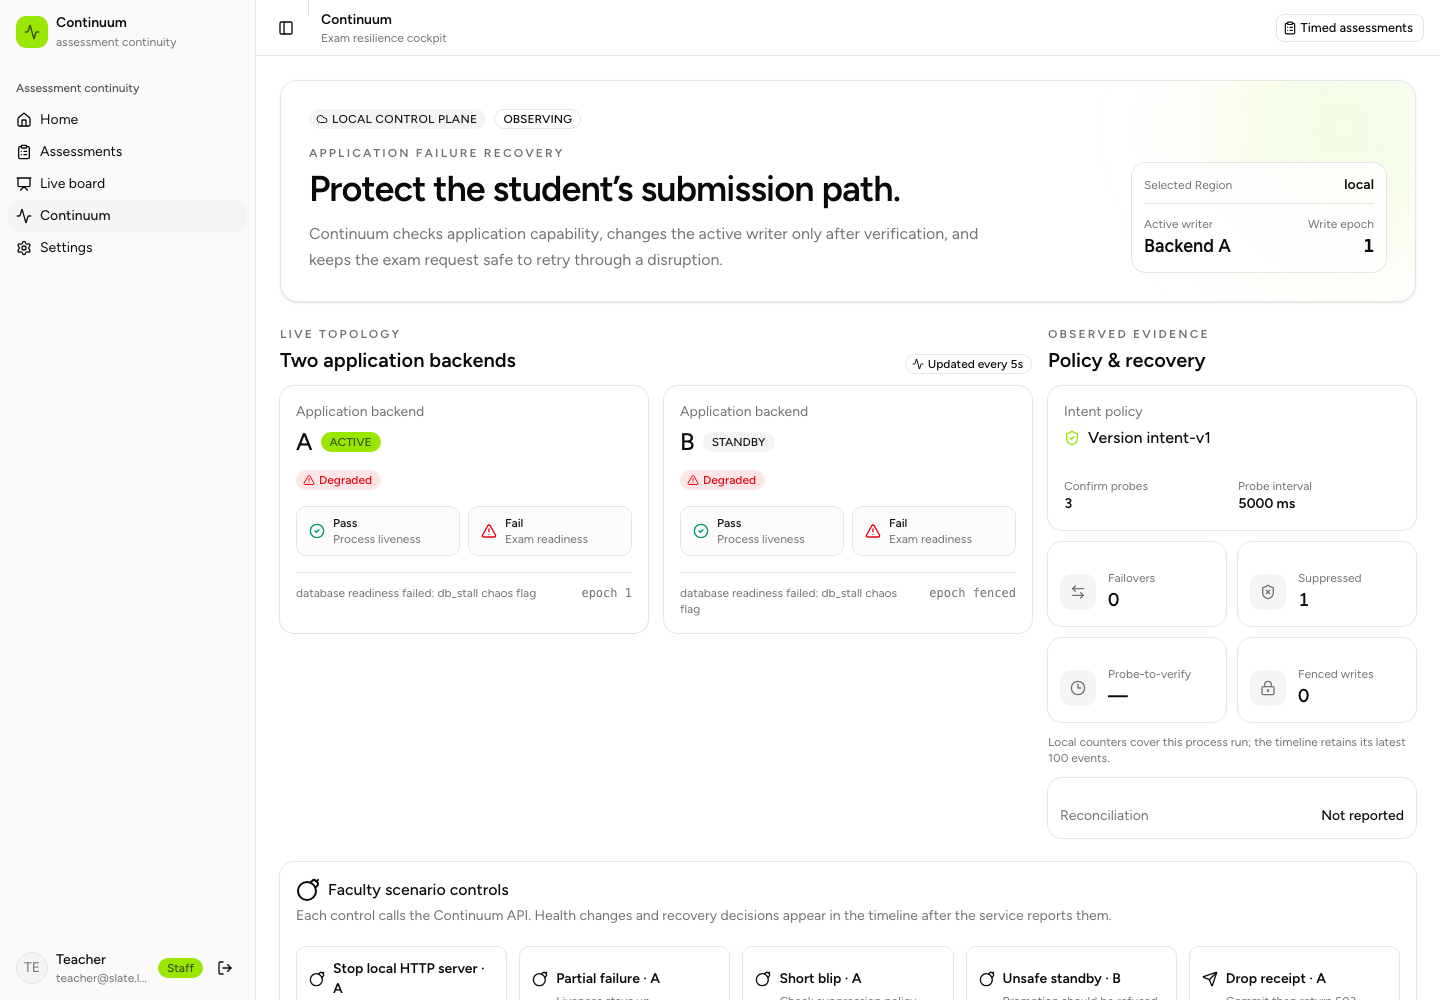
\includegraphics[width=\textwidth,trim=270bp 155bp 15bp 75bp,clip]{screenshots/recovery-unsafe-standby.png}
\caption[Local suppression when both backends are unready]{Local unsafe-standby case: both processes are alive but fail assessment readiness. Promotion is suppressed and A retains epoch 1.}\label{fig:unsafe}
\end{figure}

After clearing the faults, the active A HTTP server was stopped. Three consecutive failed probes led to B becoming active at epoch 2. The local screen reports 10,010\,ms from the first failed monitor probe to route verification. This excludes the earlier wait for that first probe and is separate from the AWS recovery measurement.

\begin{figure}[htbp]\centering
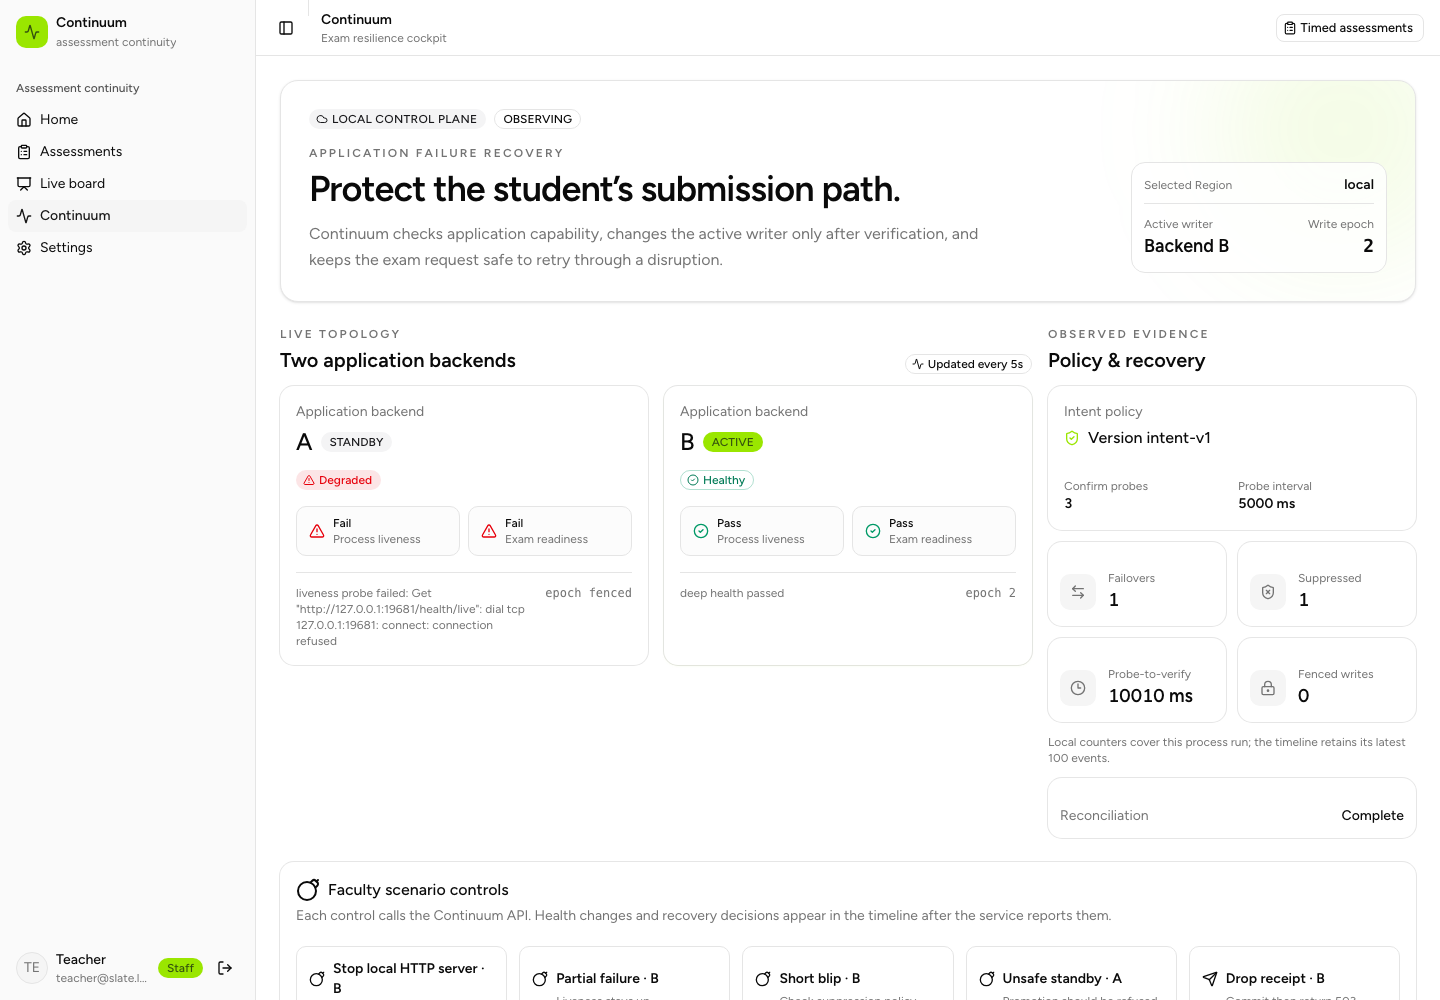
\includegraphics[width=\textwidth,trim=270bp 155bp 15bp 75bp,clip]{screenshots/recovery-local-promoted.png}
\caption[Local recovery to backend B at epoch 2]{Local recovery after stopping A's HTTP server: B is healthy and active at epoch 2; reconciliation is complete.}\label{fig:local-promoted}
\end{figure}

\begin{figure}[htbp]\centering
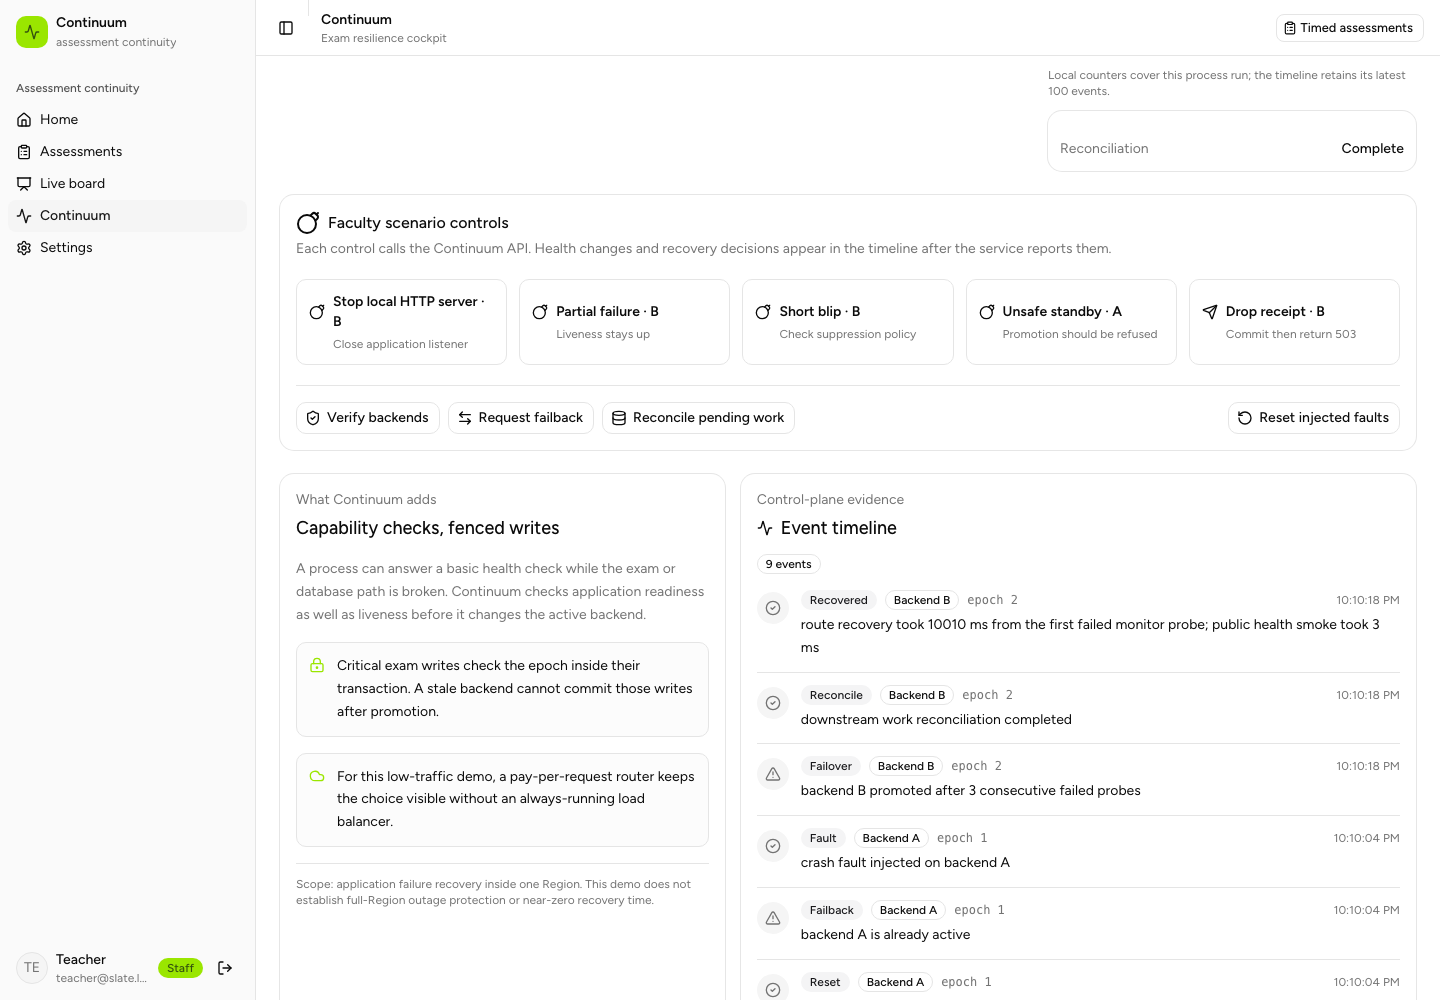
\includegraphics[width=112mm,trim=750bp 85bp 20bp 475bp,clip]{screenshots/recovery-event-timeline.png}
\caption[Local recovery event history]{Event history records the injected fault, promotion, public verification, and reconciliation. The list is ordered for operational viewing.}\label{fig:event-history}
\end{figure}

\FloatBarrier
\section{AWS Experiment Design}
The cloud rehearsal used two EC2 application instances in separate Sydney Availability Zones, a shared regional DynamoDB table, and the deployed routing and recovery services. A was initially active at epoch 1. Before the principal run, a 7.5-second transient fault recovered during confirmation, and an unsafe-standby case made both backends unready. Both suppressed promotion and retained epoch 1~\cite{cloud-run}.

The principal sequence combined a committed submission with an unavailable response:
\begin{enumerate}
\item Submit a fixed synthetic answer snapshot with a persistent request identifier. Commit succeeds, but injected response loss returns HTTP 503.
\item Request an actual stop of the active EC2 instance. Allow the scheduled monitor and workflow to determine the recovery action.
\item Observe B at epoch 2, verify public deep health, and inspect reconciliation.
\item Replay the unchanged request, then alter its payload under the same identifier and inspect the resulting conflict.
\item Independently count submission-related records and repeat reconciliation.
\end{enumerate}
This resolves one ambiguous committed outcome through a backend failure. It does not measure cohort throughput or continued writes during loss of DynamoDB.

\section{Recovery Timeline and Writer Authority}
Figure~\ref{fig:cloud-timeline} aligns events to the start of the instance-stop action. The workflow-start event appears at 41.940 seconds; promotion at 45.287 seconds, public verification at 45.470 seconds, and reconciliation at 47.970 seconds. External polling observed recovery at 50.472 seconds. These timestamps establish the sequence without identifying every internal scheduling or network delay.

\begin{figure}[htbp]\centering
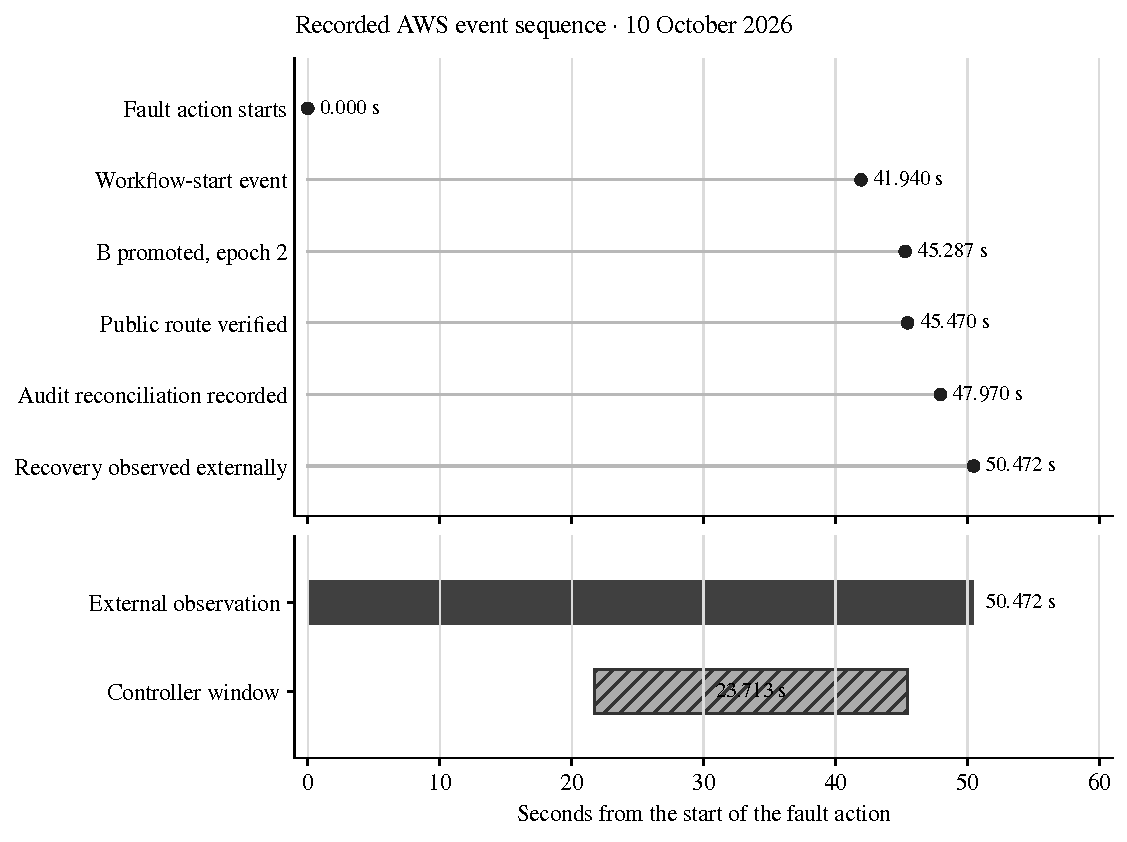
\includegraphics[width=\textwidth]{figures/cloud-timeline.pdf}
\caption[Recorded AWS event timeline and timing windows]{Recorded AWS event sequence and timing windows. The controller window's left endpoint is derived from the verification timestamp minus its recorded 23.713-second duration.}\label{fig:cloud-timeline}
\end{figure}

The external and controller intervals use different boundaries:
\begin{align}
T_{\mathrm{external}} &= t_{\mathrm{external\ observation}}-t_{\mathrm{fault\ action}}=50.472\,\mathrm{s},\\
T_{\mathrm{controller}} &= t_{\mathrm{public\ smoke}}-t_{\mathrm{check\ cycle\ start}}=23.713\,\mathrm{s}.
\end{align}
The controller interval begins before the workflow-start event because it includes monitoring and confirmation. Subtracting the durations does not isolate a single scheduling overhead: the endpoints differ, and external observation also includes polling and reconciliation. The preserved workflow result supplies the controller duration~\cite{cloud-records}.

\begin{figure}[htbp]\centering
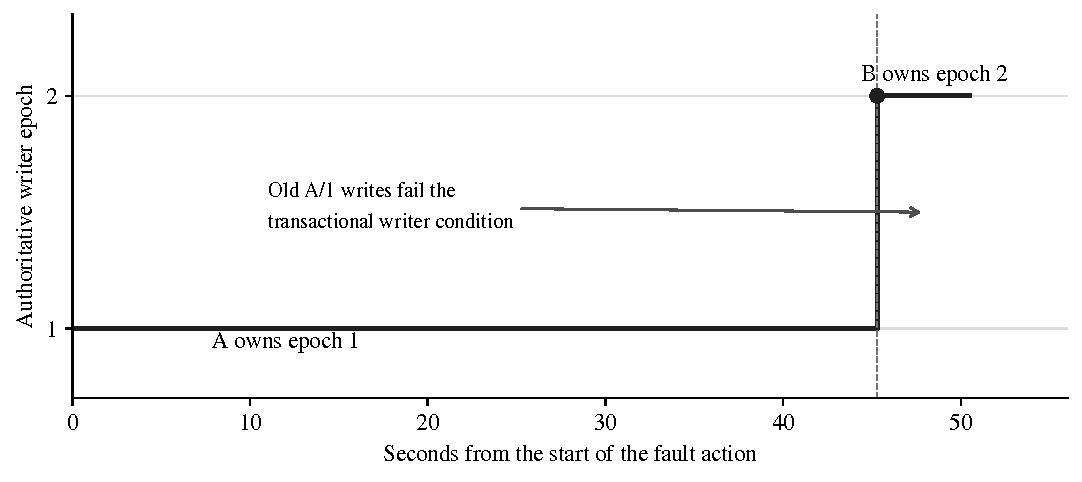
\includegraphics[width=\textwidth]{figures/writer-epoch.pdf}
\caption[Authoritative writer epoch transition]{Writer state reconstructed from the initial record and promotion event. Authority changes once from A/1 to B/2; restarting A does not grant it a newer epoch.}\label{fig:epoch-results}
\end{figure}

Figure~\ref{fig:epoch-results} represents authority, not merely process availability. An old in-flight transaction either commits before the promotion condition wins or fails the writer condition after it. Routing convergence alone would leave a period in which old A could still mutate shared data. The transactional fence closes that gap for protected writes.

\begin{figure}[htbp]\centering
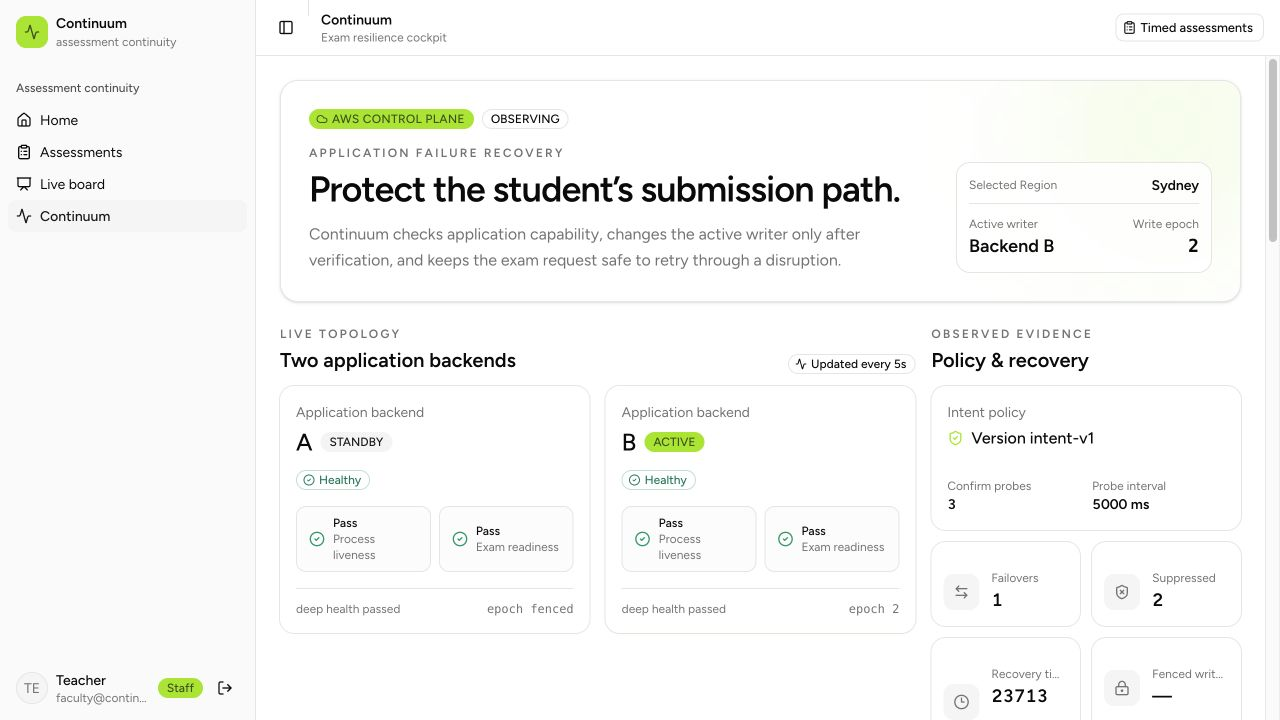
\includegraphics[width=\textwidth,trim=265bp 0bp 15bp 55bp,clip]{screenshots/cloud-recovery.png}
\caption[Recorded AWS recovery cockpit]{Preserved AWS cockpit from the cloud rehearsal, showing B active at epoch 2. This capture is separate from the new local demonstrations.}\label{fig:cloud-cockpit}
\end{figure}

\FloatBarrier
\section{Resolving the Lost Response}
The commit timestamp precedes the fault action by 1.609 seconds. Although the original request returned HTTP 503 after response loss, the exact retry returned a duplicate receipt with the original commit time. Here, duplicate means that the existing result was recovered, not that another submission was accepted.

\begin{table}[H]\centering\small
\caption{Recorded submission and replay comparison}\label{tab:receipt-comparison}
\begin{tabularx}{\textwidth}{@{}L{43mm}Y@{}}\toprule
\textbf{Field or operation} & \textbf{Recorded outcome}\\\midrule
Persistent request identifier & \texttt{cloud-6fbb0f1bc6fd4a86bdab2e9c17f33d23}\\
Original response after commit & HTTP 503 (deliberate response-loss injection)\\
Original commit timestamp & \texttt{1791652428408} milliseconds since the Unix epoch\\
Exact replay & \texttt{duplicate}; identical identifier and commit timestamp\\
Receipt scope and result & Attempt 1, version 1, score 2 of 5\\
Same identifier, changed answers & HTTP 409 conflict\\
Independent record inspection & One canonical submission, one receipt, one processed journal entry, one audit summary\\\bottomrule
\end{tabularx}\end{table}

The unchanged identifier and commit time answer the learner's question: the original submission exists despite the failed response. The changed-payload conflict establishes that the identifier cannot silently acquire another answer snapshot. Neither result follows merely from promoting a healthy standby.

\section{Reconciliation: Correctness and Work Performed}
The automatic recovery execution succeeded with one processed entry and zero conflicts. A repeated execution succeeded with zero new processed entries and zero conflicts. Independent inspection found one audit summary for the request~\cite{cloud-records}. Together, these support one logical downstream outcome for this inspected submission.

\begin{figure}[htbp]\centering
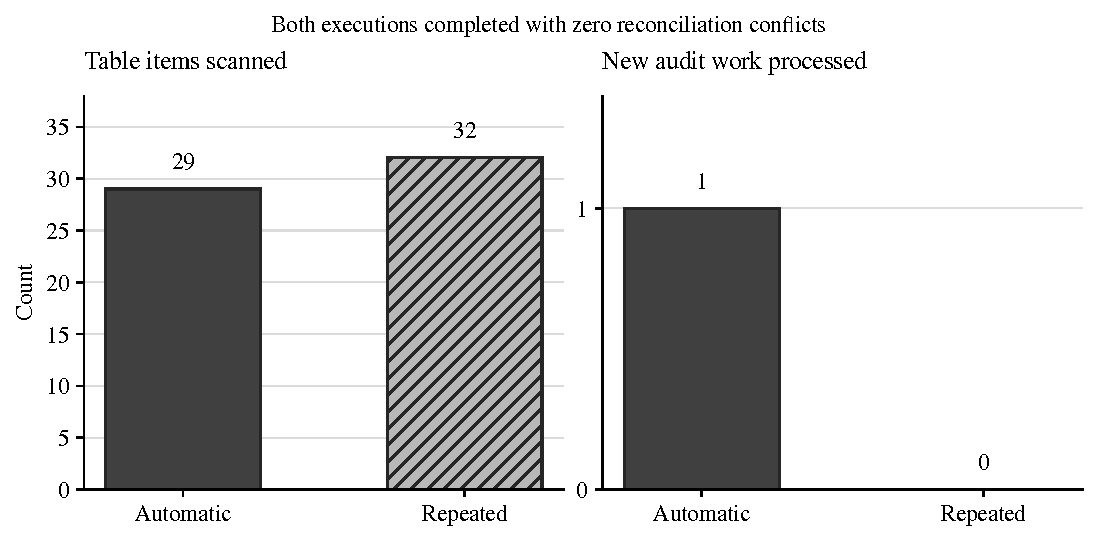
\includegraphics[width=\textwidth]{figures/reconciliation-work.pdf}
\caption[Observed reconciliation scans and new audit work]{Observed reconciliation: 29 and 32 table items scanned, with one and zero new audit outcomes. Scan count does not mean pending-submission count.}\label{fig:reconcile-work}
\end{figure}

The repeat still scanned 32 items. Idempotency prevents repeated business effects but does not make discovery free. The reconciler scans a table using an outbox filter, so \texttt{ScannedCount} can grow with unrelated data. A pending-work index or dedicated stream is a scaling improvement; this experiment does not establish that repeated scans remain efficient at institutional scale.

\section{Stale-Writer Validation}
After A restarted, a synthetic registration sent directly to A with epoch 1 returned HTTP 503 and \texttt{WRITER\_FENCED}. A strongly consistent email-index lookup found no created record~\cite{cloud-stale}. This checks stale registration specifically. Exam-submission fencing is covered by transactional storage and API tests; a stale exam submission was not sent directly to AWS in this rehearsal.



\section{Interpretation and Validity}
The strongest result combines route recovery, unchanged submission identity, and one inspected logical audit result. Suppression cases matter equally: a useful controller sometimes preserves the route rather than promotes. The local screens make decisions visible, while the AWS records establish the bounded cloud outcome.

Four limits constrain generalisation. One cloud run cannot establish mean or percentile recovery time, a production RTO, or an SLA. The workload is synthetic rather than a concurrent examination cohort. Shared DynamoDB, control services, and the selected Region remain dependencies. Finally, current-source checks and later local captures are dated separately from the preserved deployment. No data loss was observed for the inspected committed request, but this is not an unconditional zero-RPO guarantee.
